% Quick start guide
\documentclass[10pt]{beamer}

\usepackage{mathtools}

% Title page details
\title{Stochastic Calculus}
\author{Kellen Kanarios}
\institute{University of Michigan}
\date{\today}

\begin{document}

\begin{frame}
% Print the title page as the first slide
\titlepage
\end{frame}

\begin{frame}[t]
  \frametitle{Background}
  \begin{onlyenv}<1-9>
    \begin{definition}
      A real-valued random variable $X$ is a mapping $X : \Omega \to \mathbb{R}$. Here, $\Omega$ is the \textbf{sample space} and $\mathbb{P}$ is the measure of the \textbf{probability space}, such that $\mathbb{P}(\Omega) = 1$.
    \end{definition}
  \end{onlyenv}
  \begin{onlyenv}<2-5>
      \begin{block}{Note}
        Intuition for a \textbf{measure}:
        \begin{enumerate}
          \item <3-> In $\mathbb{R}$: length,
          \item <4-> In $\mathbb{R}^2$: area,
          \item <5-> In $\mathbb{R}^3$: volume.
        \end{enumerate}
      \end{block}
  \end{onlyenv}
  \begin{onlyenv}<6-9>
      \begin{block}{Definition translated into english}
        \begin{enumerate}
          \item<7->
            Unbeknownst to us, someone chooses a random $\omega \in \Omega$. Then we see the $X(\omega) \in \mathbb{R}$.
          \item<8->
            We cannot see the corresponding $\omega \in \Omega$, but the $X(\omega) \in \mathbb{R}$ gives us partial information about $\omega$.
          \item<9-> $\mathbb{P}$ tells us how likely subsets $A \subseteq \Omega$ are to occur.
        \end{enumerate}
      \end{block}
  \end{onlyenv}
  \begin{onlyenv}<10>
    \begin{example}
      Consider the case where you flip a coin. Using our previous definition, this could be described as $\Omega = \{\text{heads}, \text{tails}\}$ and \\
      \vskip 5pt
      $X(\omega) = \begin{cases}
        1, &\text{ if }\omega = \text{heads}\\
        -1, &\text{ if }\omega = \text{tails}\\
      \end{cases}$ \hspace*{10mm} where $\omega \in \Omega$. \\
      \vskip 5pt
      This would yield the familiar notation of $\mathbb{P}(X = 1) = .5$ and $\mathbb{P}(X = -1) = .5$ for a fair coin.
    \end{example} 
    \end{onlyenv}
    \begin{onlyenv}<11->
      \begin{definition}
        A \textbf{stochastic process} is a family of random variables indexed by a time parameter $t \geq 0$.
      \end{definition}
    \end{onlyenv}
    \begin{onlyenv}<12->
      \begin{example}
        A sequence of coin flips. At each time $t$ your process corresponds to a random variable (aka coinflip) $X_t$.
      \end{example}
    \end{onlyenv}
\end{frame}


\begin{frame}[t]
  \frametitle{Wiener Process}
  \begin{onlyenv}<1-5>
  \begin{definition}
    A stochastic process $W$ is called a \textbf{Wiener process} if the follow conditions hold:
    \begin{enumerate}
      \item<2-> $W_0 = 0$,
      \item<3-> The process $W$ has independent increments,
      \item<4->
          For $s < t$ the random variable $W_t - W_s$ has the Gaussian distribution $\mathcal{N}(0,t-s)$,
          \begin{figure}
            \centering
            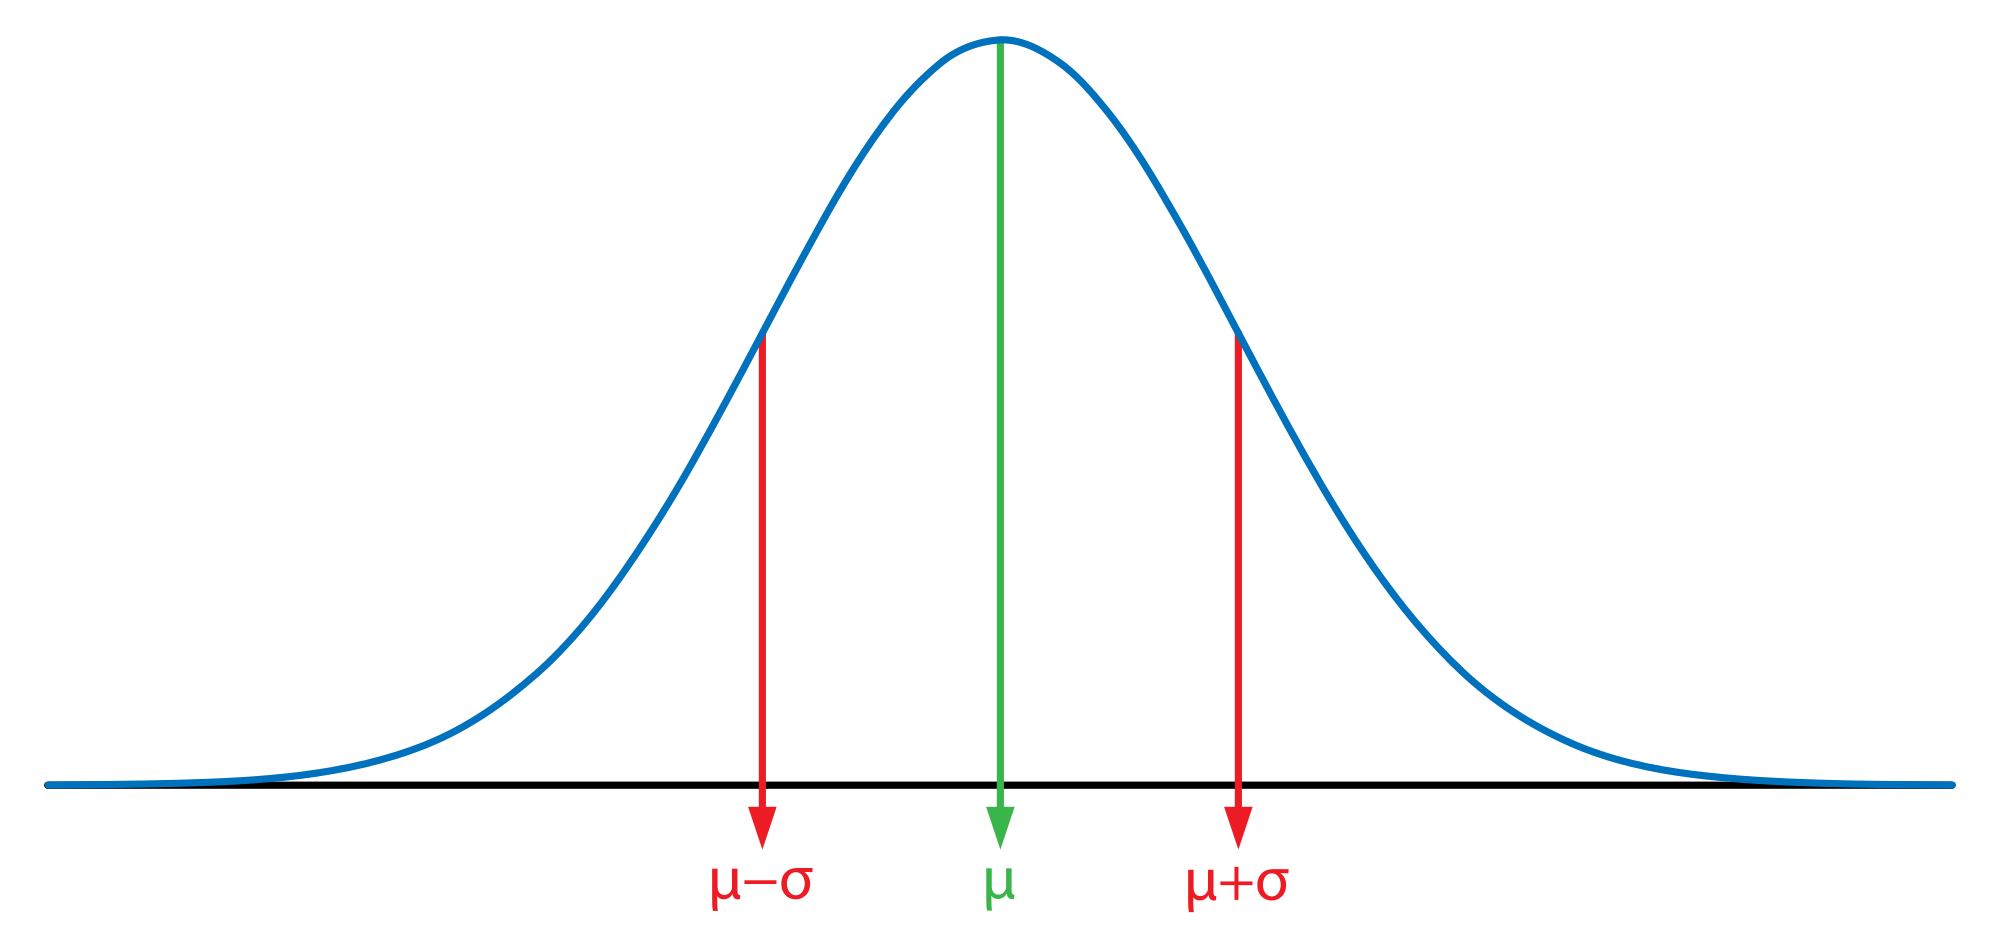
\includegraphics[width=.5\linewidth]{graphics/normal-distribution.png}
          \end{figure}
      \item<5-> $W$ has continuous trajectories.
    \end{enumerate}
  \end{definition}
  \end{onlyenv}
  \begin{onlyenv}<6->
    \begin{theorem}
      A Wiener trajectory is with probability one, nowhere differentiable, and it has locally infinite total variation.
    \end{theorem}
    \begin{figure}
      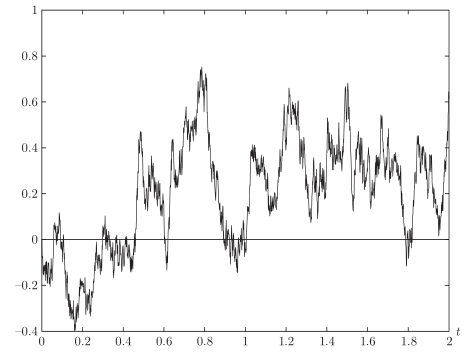
\includegraphics[scale=.45]{./graphics/wiener-trajectory.png}
      \caption{Wiener trajectory}
    \end{figure}
  \end{onlyenv}
\end{frame}

\begin{frame}[t]
  \frametitle{Quadratic Variation}
  \begin{onlyenv}<1->
    \begin{definition}
      Let $X$ be a stochastic process. Suppose $P$ is a partition of $[0,t]$ denoted $t_k$ and let $\lVert P \rVert$ be the mesh of the partition then the \textbf{quadratic variation} of $X$ is defined to be:
          \begin{align*}
            [X]_t = \lim\limits_{\lVert P \rVert \to 0} \displaystyle\sum_{k = 1}^{n}(X_{t_k} - X_{t_{k-1}})^2
          \end{align*}
    \end{definition}
  \end{onlyenv}
  \begin{onlyenv}<2->
    \begin{block}{Comments}
      Note that Quadratic Variation itself is a stochastic process. An intuitive way to think about quadratic variation is the internal clock of a process, describing how randomness accumulates over time.
    \end{block}
  \end{onlyenv}
\end{frame}


\begin{frame}[t]
  \frametitle{The Stochastic Integral}
  \begin{onlyenv}<1-3>
    \begin{block}{The Problem}
      Integrals of the form $\displaystyle\int_{0}^{t}g_s dW_s$ for some stochastic process $g_s$.
    \end{block}
  \end{onlyenv}
  \begin{onlyenv}<2-3>
    \begin{block}{Possible Solution 1}
      Try to define like the Riemman Integral
      \begin{enumerate}
        \item<2-> $\displaystyle\sum_{k = 1}^{n}g_s(W_{t_{k+1}} - W_{t_{k}})$
        \item<3-> Not possible due to locally unbounded variation of a Wiener Process.
      \end{enumerate}
    \end{block}
  \end{onlyenv}
  \begin{onlyenv}<4-5>
    \begin{definition}
      A stochastic process is \textbf{simple} on $[a,b]$ when there exists deterministic points in time $a = t_0 < t_1 < \dots < t_n = b$ such that $g_s = g_{t_k}$ for all $s \in [t_k, t_{k+1}]$.
    \end{definition}
  \end{onlyenv}
  \begin{onlyenv}<5>
      \begin{block}{Real Solution}
        Now we can define the stochastic integral by
        \begin{align*}
          \displaystyle\int_{a}^{b}g_s dW_s = \displaystyle\sum_{k = 0}^{n - 1}g_{t_k}[W_{t_{k+1}} - W_{t_{k}}]
        \end{align*}
        For some simple stochastic process $g_s$.
      \end{block}
  \end{onlyenv}
  \begin{onlyenv}<6->
    \begin{block}{How do we generalize this?}
    \end{block}
  \end{onlyenv}
\end{frame}

\begin{frame}[t]
  \frametitle{Quadratic Variation of Wiener Process}
    \begin{onlyenv}<1-3>
    \begin{theorem}
      Quadratic variation of a Wiener Process on the interval $[0,t]$ is $t$.
    \end{theorem}
    \end{onlyenv}
    \begin{onlyenv}<2-3>
      \begin{block}{Proof.}
        Let $P = \{0 = t_0 \leq t_1 \leq \dots \leq t_m = t\}$ be a partition of the interval $[0,t]$. Then the quadratic variation on $P$ is
        \begin{align*}
          [W]^{P}_{t} &= \displaystyle\sum_{k = 1}^{m}(W_{t_k} - W_{t_{k-1}})^2 
        \end{align*}
        \onslide<3->{
          Therefore,
          \begin{align*}
            \mathbb{E}\left[[W]^{P}_{t}\right] &= \displaystyle\sum_{k = 1}^{m}\mathbb{E}\left[(W_{t_k} - W_{t_{k-1}})^2\right]
          \end{align*}
        }
      \end{block}
    \end{onlyenv}
    \begin{onlyenv}<4-8>
      \begin{block}{Stats break}
        \onslide<5->{
        It is a well known fact that 
        \begin{align*}
          Var(X) = \mathbb{E}(X^2) - (\mathbb{E}(X))^2
        \end{align*}
        }
        \onslide<6->{
        Since $W_{t_{k}} - W_{t_{k-1}} \in \mathcal{N}(0, t_{k} - t_{k-1})$, 
        \begin{align*}
          \mathbb{E}(W_{t_{k}} - W_{t_{k-1}}) = 0
        \end{align*}
        }
        \onslide<7->{ 
        It follows that 
        \begin{align*}
          (\mathbb{E}(W_{t_{k}} - W_{t_{k-1}})^2) = 0 
        \end{align*}
        }
        \onslide<8->{
        Thus, $Var(W_{t_{k}} - W_{t_{k-1}}) = E((W_{t_{k}} - W_{t_{k-1}})^2)$.
        }
      \end{block}
    \end{onlyenv}
    \begin{onlyenv}<9-11>
      \begin{proof}
        Since $\mathbb{E}[(W_{t_{k}} - W_{t_{k-1}})^2] = Var\left[W_{t_{k}} - W_{t_{k-1}}]$, we can write:
      \begin{align*}
        \mathbb{E}\left[[W]^{P}_{t}\right] &= \displaystyle\sum_{k = 1}^{m}Var\left[W_{t_k} - W_{t_{k-1}}\right]
      \end{align*}
      \onslide<10->{
        Using $W_{t_k} - W_{t_{k-1}} \in \mathcal{N}(0, t_k - t_{k-1})$:
        \begin{align*}
          \mathbb{E}\left[[W]^{P}_{t}\right] &= \displaystyle\sum_{k = 1}^{m}(t_{k} - t_{k-1}) \\
          &= t
        \end{align*}
      }
      \onslide<11->{ 
        Now we must show $\mathbb{E}([W]^{P}_{t}) = [W]_t = t$.
      }
      \end{proof}
    \end{onlyenv}
    \begin{onlyenv}<12->
      \begin{block}{Implications}
        This motivates us to write 
        \begin{align*}
          \int\limits_{0}^{t}(dW_t)^2 = t
        \end{align*}
        Or equivalently,
        \begin{align*}
          (dW_t)^2 = dt
        \end{align*}
        This is one third of something called Ito's multiplication table.
      \end{block}
  \end{onlyenv}
\end{frame}

\begin{frame}[t]
  \frametitle{Ito's Multiplication Table}
  \begin{onlyenv}<1-4>
  \begin{definition}
    \textbf{Ito's multiplication table} is: 
    \begin{center}
      \renewcommand\arraystretch{1.3}
      \setlength\doublerulesep{0pt}
      \begin{tabular}{r||*{4}{2|}}
       & $dt$ & $dW_t$ \\
      \hline\hline
      $dt$ & 0 & 0 \\ 
      \hline
      $dW_t$ & 0 & $dt$ \\ 
      \end{tabular}
    \end{center} 
    \end{definition}
    We have already shown the only interesting result: $(dW_t)^2 = dt$.
  \end{onlyenv}
  \begin{onlyenv}<2-4>
    \begin{proof}[Quick sketch.]
      Suppose you are integrating on the interval $[a,b]$. Partition [a,b] into $N$ increments. Then $dt \sim \frac{1}{N}$ and $(dt)^2 \sim \frac{1}{N^2}$. It follows that:
      \begin{align*}
        \displaystyle\sum_{i = 1}^{N}\frac{1}{N^2} &= \frac{1}{N} \\
        \lim\limits_{N \to \infty}\displaystyle\sum_{i = 1}^{N}\frac{1}{N^2} &= \lim\limits_{N \to \infty} \frac{1}{N} = \displaystyle\int_{a}^{b}(dt)^2 = 0
      \end{align*}
    \end{proof}
  \end{onlyenv}
  \begin{onlyenv}<5->
    \begin{proof}[Quick sketch.]
      Similarly, suppose you are integrating on the interval $[a,b]$. Partition [a,b] into $N$ increments. Since $dW_t = \sqrt{dt}$, $dt \sim \frac{1}{N}$ and $(dt) (dW_t) \sim \frac{1}{N^{3/2}}$. It follows that:
      \begin{align*}
        \displaystyle\sum_{i = 1}^{N}\frac{1}{N^{3/2}} &= \frac{1}{N^{1/2}} \\
        \lim\limits_{N \to \infty}\displaystyle\sum_{i = 1}^{N}\frac{1}{N^{3/2}} &= \lim\limits_{N \to \infty} \frac{1}{N^{1/2}} = \displaystyle\int_{a}^{b}(dt)(dW_t) = 0
      \end{align*}
    \end{proof}
  \end{onlyenv}
  \begin{onlyenv}<6->
    This completes the multiplication table and provides the foundation for introducing Ito's lemma.
  \end{onlyenv}
\end{frame}

\begin{frame}[t]
  \frametitle{Ito's Lemma}
  \begin{onlyenv}<1>
  \begin{theorem}[Ito's formula]
    Assume that process $X$ has a stochastic differential given by 
    \begin{align*}
      dX_t = \mu_t dt + \sigma_t dW_t
    \end{align*}
    Define the process $Z$ by $Z(t) = f(t, X_t)$. Then $Z$ has a stochastic differential given by
    \begin{align*}
      df(t, X_t) &= \left\{\frac{\partial f}{\partial t}(t, X_t) + \mu_t \frac{\partial f}{\partial x}(t,X_t) + \frac{1}{2}\sigma^2_t\frac{\partial^2 f}{\partial x^2}(t,X_t)\right\}dt + \sigma \frac{\partial f}{\partial x}(t, X_t)dW_t
    \end{align*}
  \end{theorem}
  \end{onlyenv}
  \begin{onlyenv}<2-6>
    \begin{block}{Heuristic proof.}
      \onslide<3-6>{
      Using $f$ from the theorem, we will consider the second order Taylor expansion:
      \begin{align*}
        df = \frac{\partial f}{\partial t}dt + \frac{\partial f}{\partial x}dX_t + \frac{1}{2}\frac{\partial^2 f}{\partial x ^2}(dX_t)^2 + \frac{1}{2}\frac{\partial^2 f}{\partial t^2}(dt)^2 + \frac{\partial^2 f}{\partial t \partial x}dt dX_t.
      \end{align*}
      }
      \onslide<4-6>{
      By definition we have
      \begin{align*}
        dX_t = \mu_t dt + \sigma_t dW_t
      \end{align*}
      }
      \onslide<5-6>{
      so, we obtain
      \begin{align*}
        (dX_t)^2 = \mu^2_t(dt)^2 + 2\mu_t \sigma_t(dt)(dW_t) + \sigma^2_t(dW_t)^2,
      \end{align*}
      }
      \onslide<6>{
      From Ito's multiplication table we have:
      \begin{align*}
        (dX_t)^2 = \sigma^2_t dt
      \end{align*}
      }
    \end{block}
  \end{onlyenv}
  \begin{onlyenv}<7->
    \begin{proof}[Heuristic proof cont.]
    \onslide<8->{
      Substituting back for $(dX_t)^2$,
      \begin{align*}
        df = \frac{\partial f}{\partial t}dt + \frac{\partial f}{\partial x}dX_t + \frac{1}{2}\frac{\partial^2 f}{\partial x ^2}(\sigma^2_t)(dt) + \frac{1}{2}\frac{\partial^2 f}{\partial t^2}(dt)^2 + \frac{\partial^2 f}{\partial t \partial x}dt dX_t.
      \end{align*}
    }
    \onslide<9->{
      Applying Ito's multiplication table one more time,
      \begin{align*}
        df = \frac{\partial f}{\partial t}dt + \frac{\partial f}{\partial x}dX_t + \frac{1}{2}\frac{\partial^2 f}{\partial x ^2}(\sigma^2_t)(dt) + \frac{\partial^2 f}{\partial t \partial x}dt dX_t.
      \end{align*}
    }
    \onslide<10->{
      Now substituing in $(dX_t)$,
      \begin{align*}
        df &= \frac{\partial f}{\partial t}dt + \frac{\partial f}{\partial x}(\mu_t dt + \sigma_t dW_t) + \frac{1}{2}\frac{\partial^2 f}{\partial x ^2}(\sigma^2_t)(dt) + \frac{\partial^2 f}{\partial t \partial x}(\mu_t dt + \sigma_t dW_t)dt. \\
        &= \left\{\frac{\partial f}{\partial t}(t, X_t) + \mu_t \frac{\partial f}{\partial x}(t,X_t) + \frac{1}{2}\sigma^2_t\frac{\partial^2 f}{\partial x^2}(t,X_t)\right\}dt + \sigma \frac{\partial f}{\partial x}(t, X_t)dW_t
      \end{align*}
    }
    \end{proof}
  \end{onlyenv}
\end{frame}

\begin{frame}[t]
  \frametitle{Geometric Brownian Motion Model}
  \begin{onlyenv}<1-2>
    \begin{definition}
      \textbf{Geometric Brownian Motion} is a stochastic process whose dynamics follow the stochastic differential equation 
      \begin{align*}
        dX_t = \alpha X_t dt + \sigma X_t dW_t \text{ for some } \alpha,\beta \in \mathbb{R}
      \end{align*}
      Where $dW_t$ is the infinitesimal increment of the Wiener process.
    \end{definition}
  \end{onlyenv}
  \begin{onlyenv}<2>
    \begin{block}{Claim:}
      The closed form of Geometric Brownian Motion is:
      \begin{align*}
        dX_t = X_0 e^{(\mu - \frac{\sigma^2}{2})dt + \sigma dW_t}
      \end{align*}
    \end{block}
  \end{onlyenv}
  \begin{onlyenv}<3-6>
    \begin{block}{Proof.}
      Assume $X_t$ follows a Geometric Brownian Motion. Using Ito's lemma,
      \begin{align*}
        d\ln(X_t) = \frac{1}{X_t}dX_t - \frac{1}{2X_t^2}(dX_t)^2
      \end{align*}
      \onslide<4->{
        From our definition of Geometric Brownian Motion,
        \begin{align*}
          d\ln(X_t) = \frac{1}{X_t}(\mu X_t dt + \sigma X_t dW_t) - \frac{1}{2X_t^2}(\mu X_t dt + \sigma X_t dW_t)^2 
        \end{align*}
      }
      \onslide<5->{
        Note that:
        \begin{align*}
          (\mu X_t dt + \sigma X_t dW_t)^2 &= X_t^2(\mu^2dt^2 + \sigma^2dW_t^2 + 2\mu \sigma dtdW_t)
        \end{align*}
      }
  % \end{onlyenv}
      \onslide<6->{
        From Ito's multiplication table, $(dt)^2 = 0 = (dt)(dW_t)$ and $(dW_t)^2 = dt$ such that
        \begin{align*}
          (\mu X_t dt + \sigma X_t dW_t)^2 &= X_t^2 \sigma^2 dt
        \end{align*}
      }
    \end{block}
  \end{onlyenv}
  \begin{onlyenv}<7->
    \begin{proof}
        Substituting back,
        \begin{align*}
          d\ln(X_t) &= (\mu dt + \sigma dW_t) - \frac{1}{2X_t^2}(X_t^2 \sigma^2 dt) \\
          &= (\mu - \frac{\sigma^2}{2})dt + \sigma dW_t.
        \end{align*}
        \onslide<8->{ 
        It follows that $dX_t = e^{(\mu - \frac{\sigma^2}{2})dt + \sigma dW_t}$
        }
    \end{proof}
  \end{onlyenv}
\end{frame}

\end{document}
